%TC:macro \todo [option:0,0]
\documentclass[12pt]{article}

\usepackage[utf8]{inputenc}
\usepackage[T1]{fontenc}
\usepackage[margin=1in]{geometry}
\usepackage{setspace}
\usepackage[colorlinks=true,linkcolor=blue,citecolor=blue,urlcolor=blue]{hyperref}
\usepackage{titlesec}
\usepackage{mathptmx} % Times Roman font
\usepackage{amsmath}  % for \text command in math mode
\usepackage{graphicx}
\usepackage{wrapfig}
\usepackage[section]{placeins}
\usepackage[font=small,labelfont=bf]{caption}
\usepackage[numbers,sort&compress]{natbib}
\usepackage[disable,textsize=footnotesize,color=yellow!40]{todonotes}
\usepackage{catchfile}

% Automatic word count via texcount (run by latexmk; no -shell-escape needed).
% Counts body text only; excludes title block, captions, todos, and references.
\newcommand{\wordcount}{%
  \IfFileExists{\jobname.wordcount}%
    {\CatchFileDef{\thewordcount}{\jobname.wordcount}{\endlinechar=-1}%
     \thewordcount}%
    {[word count unavailable]}%
}

% Compact section formatting to maximize space
\titleformat{\section}{\normalfont\bfseries\large}{\thesection.}{0.5em}{}
\titleformat{\subsection}{\normalfont\bfseries\normalsize}{\thesubsection.}{0.5em}{}
\titlespacing*{\section}{0pt}{1.5ex plus 0.5ex minus 0.2ex}{0.8ex plus 0.2ex}
\titlespacing*{\subsection}{0pt}{1.0ex plus 0.3ex minus 0.2ex}{0.5ex plus 0.1ex}

% No page numbers on first page, numbers on subsequent pages
\pagestyle{plain}

\begin{document}

\doublespacing

%TC:ignore
\begin{center}
{\large \textbf{Pitzer Ion-Interaction Framework for Predicting Sulfide-Mineral Precipitation from Petroleum-Derived H$_2$S and Organic Acids in Produced-Water Brines}}\\[0.3em]
{\small Sterling G. Baird, Department of Mechanical Engineering, Brigham Young University}
\end{center}

\begin{abstract}
\noindent
Sulfide mineral scales form when petroleum-derived H$_2$S---generated by thermochemical and bacterial sulfate reduction of crude oil hydrocarbons---reacts with dissolved Fe$^{2+}$ and Pb$^{2+}$ in produced waters, depositing iron sulfide and lead sulfide that restrict flow and foul equipment. These produced waters also contain petroleum-derived organic acids (acetic, propionic) from thermal maturation of kerogen, which modify sulfide precipitation through pH buffering and metal complexation. The Pitzer ion-interaction model predicts ion activities in concentrated electrolytes, yet parameterization for these interactions remains incomplete. Binary parameters ($\beta^{(0)}$, $\beta^{(1)}$, $C^\phi$) for Fe$^{2+}$--HS$^-$ and Pb$^{2+}$--HS$^-$ are absent from standard databases, and Pitzer parameters for metal--organic acid interactions (Fe$^{2+}$--acetate, Pb$^{2+}$--acetate, Fe$^{2+}$--propionate, Pb$^{2+}$--propionate) have never been determined---$\sim$48 unmeasured parameters that prevent rigorous prediction of sulfide-mineral solubility in produced-water brines.

We propose to determine these parameters through systematic high-throughput experiments. Using an Opentrons OT-2 platform, we will map FeS and PbS precipitation boundaries across $\sim$30{,}000 experiments spanning metal-ion, sulfide, and organic acid concentrations, ionic strength (0.5--5~molal), pH (4--9), and temperature (25--90~$^\circ$C). Organic acids are introduced as sodium salts to independently vary concentration. Latin hypercube sampling provides broad coverage; a staged active learning strategy adaptively targets informative conditions near precipitation boundaries. Results are compared to PHREEQC Pitzer-model predictions; where deviations exceed $\pm$0.2 saturation-index units, new parameters are regressed via nonlinear least-squares fitting and validated through cross-validation. The resulting framework fills a critical gap in electrolyte thermodynamics, delivering validated parameters for petroleum-industry scale prediction tools and enabling accurate prediction of how petroleum-derived compounds govern sulfide-scale formation in complex brines.
\end{abstract}
%TC:endignore

\newpage

\section{Introduction}

\begin{wrapfigure}{r}{0.55\textwidth}
\centering
\vspace{-1.5em}
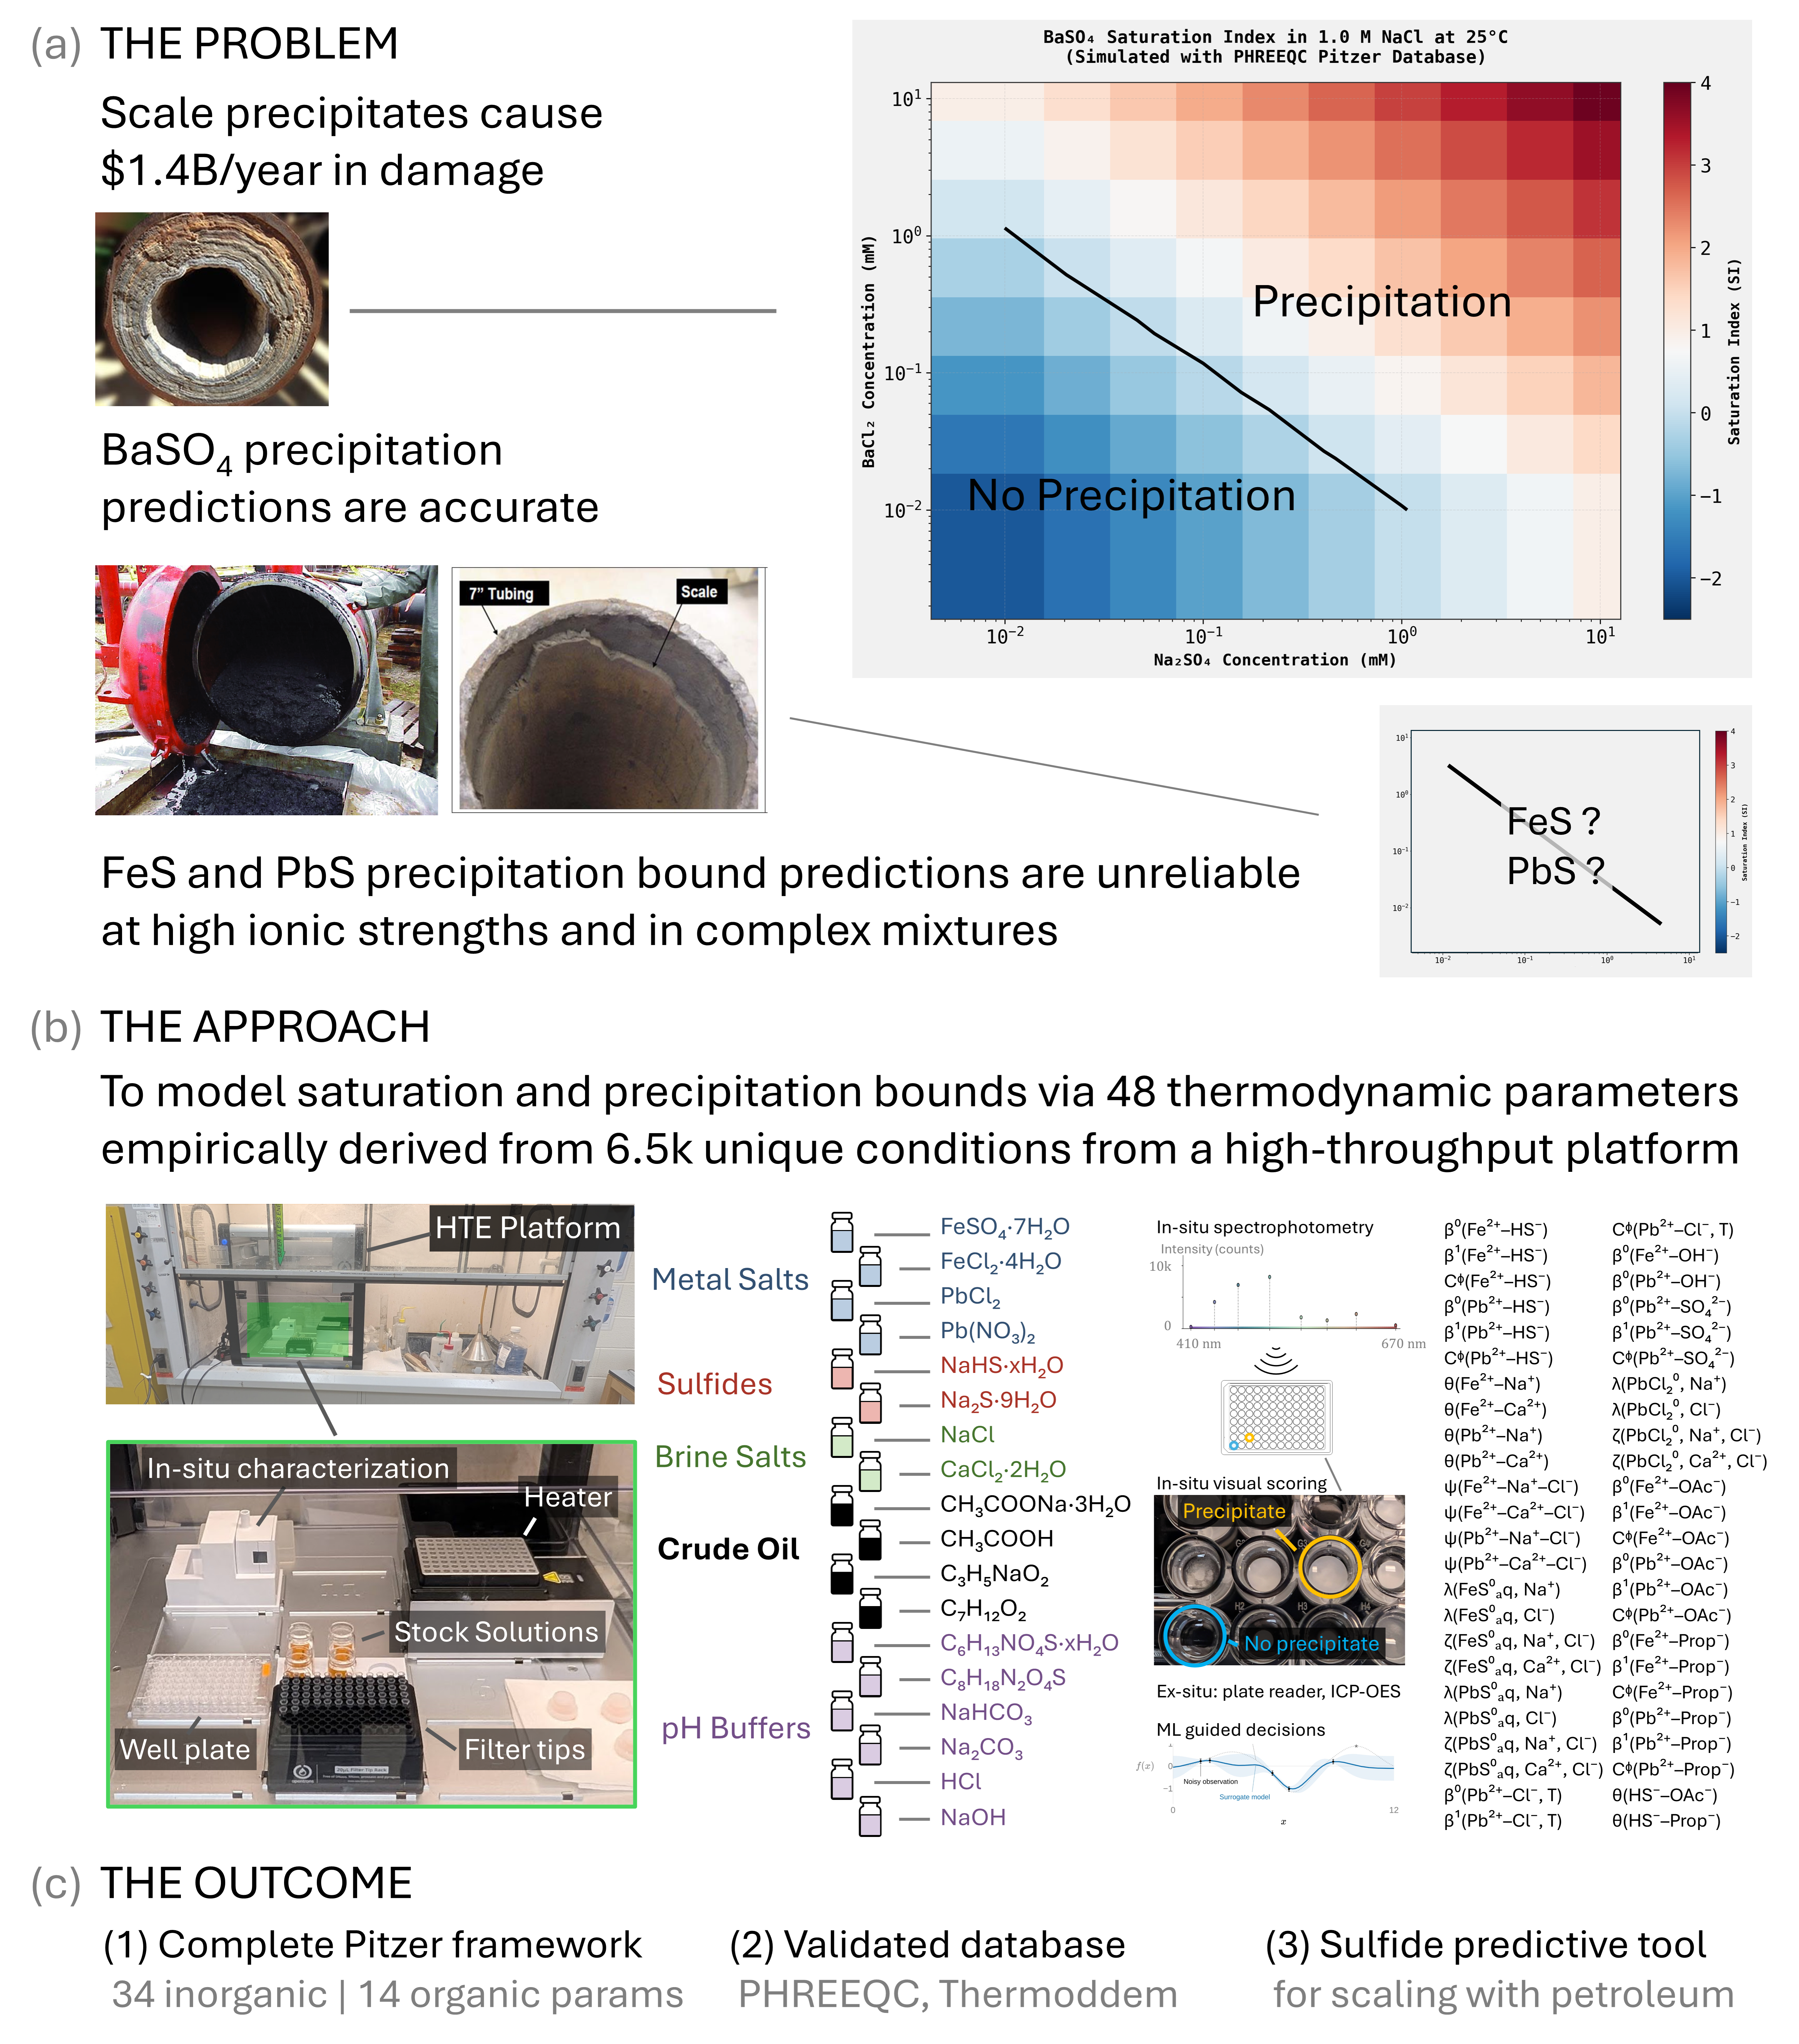
\includegraphics[width=0.54\textwidth]{problem-approach-outcome-overview.png}
\caption{Overview of the proposed Pitzer framework for petroleum-relevant sulfide chemistry. (a)~The Problem: Current databases lack $\sim$48 parameters for interactions between Fe$^{2+}$/Pb$^{2+}$ with petroleum-derived compounds (H$_2$S from TSR/BSR, and organic acids from kerogen maturation). (b)~The Approach: High-throughput experiments ($\sim$5k unique conditions per metal system, triplicates, $\sim$30k total experiments via high throughput experimentation) coupled with Pitzer model refinement through adaptive sampling. (c)~The Outcome: Complete, petroleum-relevant prediction framework via parameter sets validated for PHREEQC, Thermoddem, and ScaleSoftPitzer.}
\label{fig:overview}
\vspace{-1em}
\end{wrapfigure}

Sulfide mineral scales form when petroleum-derived H$_2$S---generated by thermochemical sulfate reduction (TSR) and bacterial sulfate reduction (BSR) of crude oil \cite{machel2001,worden1996}---reacts with dissolved Fe$^{2+}$ and Pb$^{2+}$ in produced waters, depositing iron sulfide (mackinawite) and lead sulfide (galena) that restrict flow and foul equipment \cite{kan2019,wylde2014}. These produced waters also contain petroleum-derived short-chain organic acids---predominantly acetic acid (100--10{,}000~mg/L) and propionic acid (10--1{,}000~mg/L)---released during thermal maturation of kerogen \cite{carothers1978,surdam1989}. These organic acids modify sulfide precipitation through pH buffering and metal complexation, yet their thermodynamic interactions with scale-forming metal ions are completely unparameterized.

The Pitzer ion-interaction model predicts ion activities in concentrated electrolytes through empirically determined interaction parameters \cite{kan2019} (Figure~\ref{fig:overview}). For sulfate scales, Pitzer models are well-validated to TDS exceeding 200{,}000~mg/L \cite{kan2019,shaferpeltier2020}. For sulfide scales, the parameter database is critically incomplete: Fe$^{2+}$--HS$^-$ and Pb$^{2+}$--HS$^-$ binary parameters are absent from all standard databases, higher-order mixing parameters with Na$^+$/Ca$^{2+}$ have never been determined, and Pitzer parameters for metal--organic acid interactions (Fe$^{2+}$--acetate, Pb$^{2+}$--acetate, Fe$^{2+}$--propionate, Pb$^{2+}$--propionate) do not exist \cite{wang2020,felmy2000,duan2007}. Without these parameters, Pitzer-based scale prediction codes (ScaleSoftPitzer, OLI Systems, PHREEQC) cannot model sulfide-mineral deposition in produced-water brines \cite{kan2019}. This gap persists for two reasons: sulfide measurements require strict inert-atmosphere handling (O$_2$ oxidizes both Fe$^{2+}$ and HS$^-$), making conventional single-vial experiments laborious; and the petroleum industry historically prioritized sulfate-scale parameters (BaSO$_4$, CaSO$_4$), with sulfide-scale problems gaining prominence only as sour-reservoir production increased. Determining the $\sim$48 missing parameters demands systematic variation across hundreds of conditions spanning ionic strength, temperature, and composition simultaneously---a scale of experimentation that has only recently become feasible through robotic high-throughput platforms and active-learning-guided experimental design.

This proposal constructs the first Pitzer ion-interaction framework that systematically accounts for how petroleum-derived compounds---both sulfide species and organic acids---interact with metal ions in multi-component brines. The fundamental question driving this work: \textit{What Pitzer parameters govern the interactions of petroleum-derived H$_2$S/HS$^-$ and organic acids with Fe$^{2+}$ and Pb$^{2+}$ in produced-water brines, and how do these interactions shift sulfide-mineral precipitation boundaries at high ionic strength?} Answering this question addresses a foundational gap in electrolyte thermodynamics: extending the Pitzer formalism---whose predictive success for sulfate scales is well established---to the sulfide and organic acid systems that dominate sour petroleum-production environments.

\section{Objectives and Specific Aims}

This project constructs a Pitzer framework for predicting how petroleum-derived compounds interact with metal ions during sulfide-mineral precipitation, determining $\sim$48 unmeasured interaction parameters through systematic experiments. We hypothesize that \textbf{accurate prediction of FeS and PbS precipitation boundaries in produced-water brines requires both (1)~the 34 inorganic metal--sulfide Pitzer parameters (binary, mixing, and neutral-species terms for Fe$^{2+}$--HS$^-$ and Pb$^{2+}$--HS$^-$) and (2)~$\sim$14 additional parameters for petroleum-derived organic acid--metal interactions (Fe$^{2+}$--acetate, Pb$^{2+}$--acetate, Fe$^{2+}$--propionate, Pb$^{2+}$--propionate, and their mixing terms) that shift precipitation boundaries through competitive complexation and pH buffering}. The Pb$^{2+}$ system, for which no Pitzer parameters of any kind exist for either sulfide or organic acid interactions \cite{wang2020,felmy2000}, represents the most critical gap.

\subsection{Aim 1: Map Experimental FeS and PbS Precipitation Boundaries Across Produced-Water-Relevant Parameter Space}

We will systematically vary metal-ion concentration ([Fe$^{2+}$] and [Pb$^{2+}$]), sulfide concentration ([HS$^-$]), organic acid concentration (sodium acetate and sodium propionate, 0--5{,}000~mg/L, introduced as sodium salts to decouple from pH), ionic strength (0.5--5~molal NaCl $\pm$ CaCl$_2$), pH (4--9), and temperature (25--90~$^\circ$C) in 96-well microplates using a Latin hypercube sampling design and an automated platform (Figure~\ref{fig:aim1}). Precipitation is detected via microplate-reader absorbance and visual scoring. The deliverable is approximately 30,000 individual measurements ($\sim$5,000 unique conditions $\times$ triplicates per metal system), combining space-filling sampling with adaptive Bayesian-optimization-guided follow-up (see below). An exploratory subset of $\sim$100 experiments using cyclohexane carboxylic acid (a model naphthenic acid) will test framework applicability to cyclic petroleum-derived organic acids.

\subsection{Aim 2: Quantify Deviations Between Experimental Boundaries and Pitzer-Model Predictions, and Regress New Interaction Parameters}

We will compute saturation indices using PHREEQC (Figure~\ref{fig:aim2}) and compare to observations. Where deviations exceed $\pm$0.2~SI, $\sim$48 Pitzer parameters---34 for inorganic metal--sulfide interactions plus $\sim$14 for metal--organic acid interactions---will be regressed via weighted least-squares and validated. Deliverable: validated parameters for Fe$^{2+}$--HS$^-$, Pb$^{2+}$--HS$^-$, and metal--organic acid systems in NaCl--CaCl$_2$ brines, suitable for PHREEQC \texttt{pitzer.dat}, gebo \cite{bozau2013}, Thermoddem, and ScaleSoftPitzer databases.

\section{Background and Significance}

\subsection{Sulfide Scales in Petroleum Production}

Sulfide scales form when petroleum-derived H$_2$S---generated by thermochemical sulfate reduction (TSR) and bacterial sulfate reduction (BSR) of crude oil \cite{machel2001,worden1996}---reacts with dissolved metals in produced waters. FeS precipitates at pH~6.5 with mg/L iron levels; PbS forms in high-temperature reservoirs \cite{wylde2014,alharbi2017}. These produced waters simultaneously contain petroleum-derived organic acids---acetic acid (100--10{,}000~mg/L) and propionic acid (10--1{,}000~mg/L)---from thermal maturation of kerogen \cite{carothers1978,surdam1989}, which modify sulfide precipitation through pH buffering and metal complexation, yet their Pitzer parameters with Fe$^{2+}$ and Pb$^{2+}$ are entirely absent from thermodynamic databases.

\subsection{Pitzer Activity-Coefficient Models and Their Limitations}

The Pitzer formalism extends Debye--H\"uckel theory using binary and ternary ion-interaction parameters \cite{kan2019}. For BaSO$_4$, extensive measurements enable accurate predictions to $I = 5$--6~molal, making Pitzer-based codes (PHREEQC, ScaleSoftPitzer) widely adopted for sulfate-scale prediction \cite{kan2019,shaferpeltier2020}. The BaSO$_4$ system demonstrates a general principle: once accurate Pitzer parameters exist, reliable thermodynamic prediction follows. For sulfide minerals, no equivalent predictive capability exists.

PHREEQC \texttt{pitzer.dat} contains Fe$^{2+}$ parameters only for Cl$^-$ and SO$_4^{2-}$, with zero Pb$^{2+}$ parameters \cite{wang2020}. Binary and mixing parameters for Fe$^{2+}$--HS$^-$ and Pb$^{2+}$--HS$^-$ are absent from Thermoddem and other databases. Bozau's ``gebo'' extension \cite{bozau2013} and Appelo's high-temperature database \cite{appelo2015} likewise omit metal--sulfide Pitzer coefficients, representing a fundamental data gap requiring new experimental measurements.

Mackinawite $K_{\text{sp}}$ values span $10^{-3.6}$--$10^{-4.65}$ \cite{wylde2014,wang2020}. Existing models rely on Debye--H\"uckel estimates at high ionic strength \cite{wang2020}, and Pitzer predictions fail above $I \approx 2$~molal \cite{felmy2000,alharbi2017}.

Binary and mixing Pitzer parameters for Fe$^{2+}$--HS$^-$ and Pb$^{2+}$--HS$^-$ systems remain unmeasured---34 inorganic parameters including temperature-dependent and neutral-species terms---and an additional $\sim$14 metal--organic acid parameters have never been determined (Aim~2). This gap persists across all database extensions \cite{bozau2013,appelo2015}. Accurate modeling requires coupling Pitzer calculations with metal--chloride, metal--sulfide, and metal--organic acid interactions \cite{kan2019,felmy2000}.

\subsection{Automated High-Throughput Precipitation Screening}

Robotic turbidity screening in 96-well microplates has been validated for precipitation detection in pharmaceutical \cite{dehring2004,petrusevska2013} and materials science contexts, where OT-2 robots have automated high-throughput co-precipitation screening at $>$100 samples per day \cite{velasco2021,kumbhakar2023,schuetzke2023}. However, measuring the thermodynamic data needed to parameterize sulfide-scale models requires systematic variation of ionic strength, temperature, and composition across hundreds of conditions---far exceeding the capacity of conventional NACE static bottle tests ($\sim$12 simultaneous samples) \cite{baugh2012}.

\textbf{Safety and environmental controls.} All sulfide and lead experiments will be conducted with the OT-2 housed inside a chemical fume hood, with adhesive plate seals applied immediately after dispensing to minimize H$_2$S off-gassing. Working at pH~$\geq$~8 ensures HS$^-$ dominance and negligible H$_2$S partial pressure. Environmental monitoring includes continuous H$_2$S gas detection and temperature/humidity logging. Elevated-temperature experiments (60--90~$^\circ$C) use sealed glass vials. Sodium acetate and sodium propionate are low-hazard reagents requiring only standard PPE. For Fe$^{2+}$ campaigns, the OT-2 will be placed inside an N$_2$ glovebox (being procured from PI startup funds) to prevent oxidation; the PI has prior experience handling hazardous chemicals including battery electrolytes, concentrated nitric acid, saturated KOH, and reactive nanomaterials.

\section{Research Plan}

\subsection{Aim 1: Experimental Precipitation Boundary Mapping}

\begin{wrapfigure}{r}{0.6\textwidth}
\centering
\vspace{-1.5em}
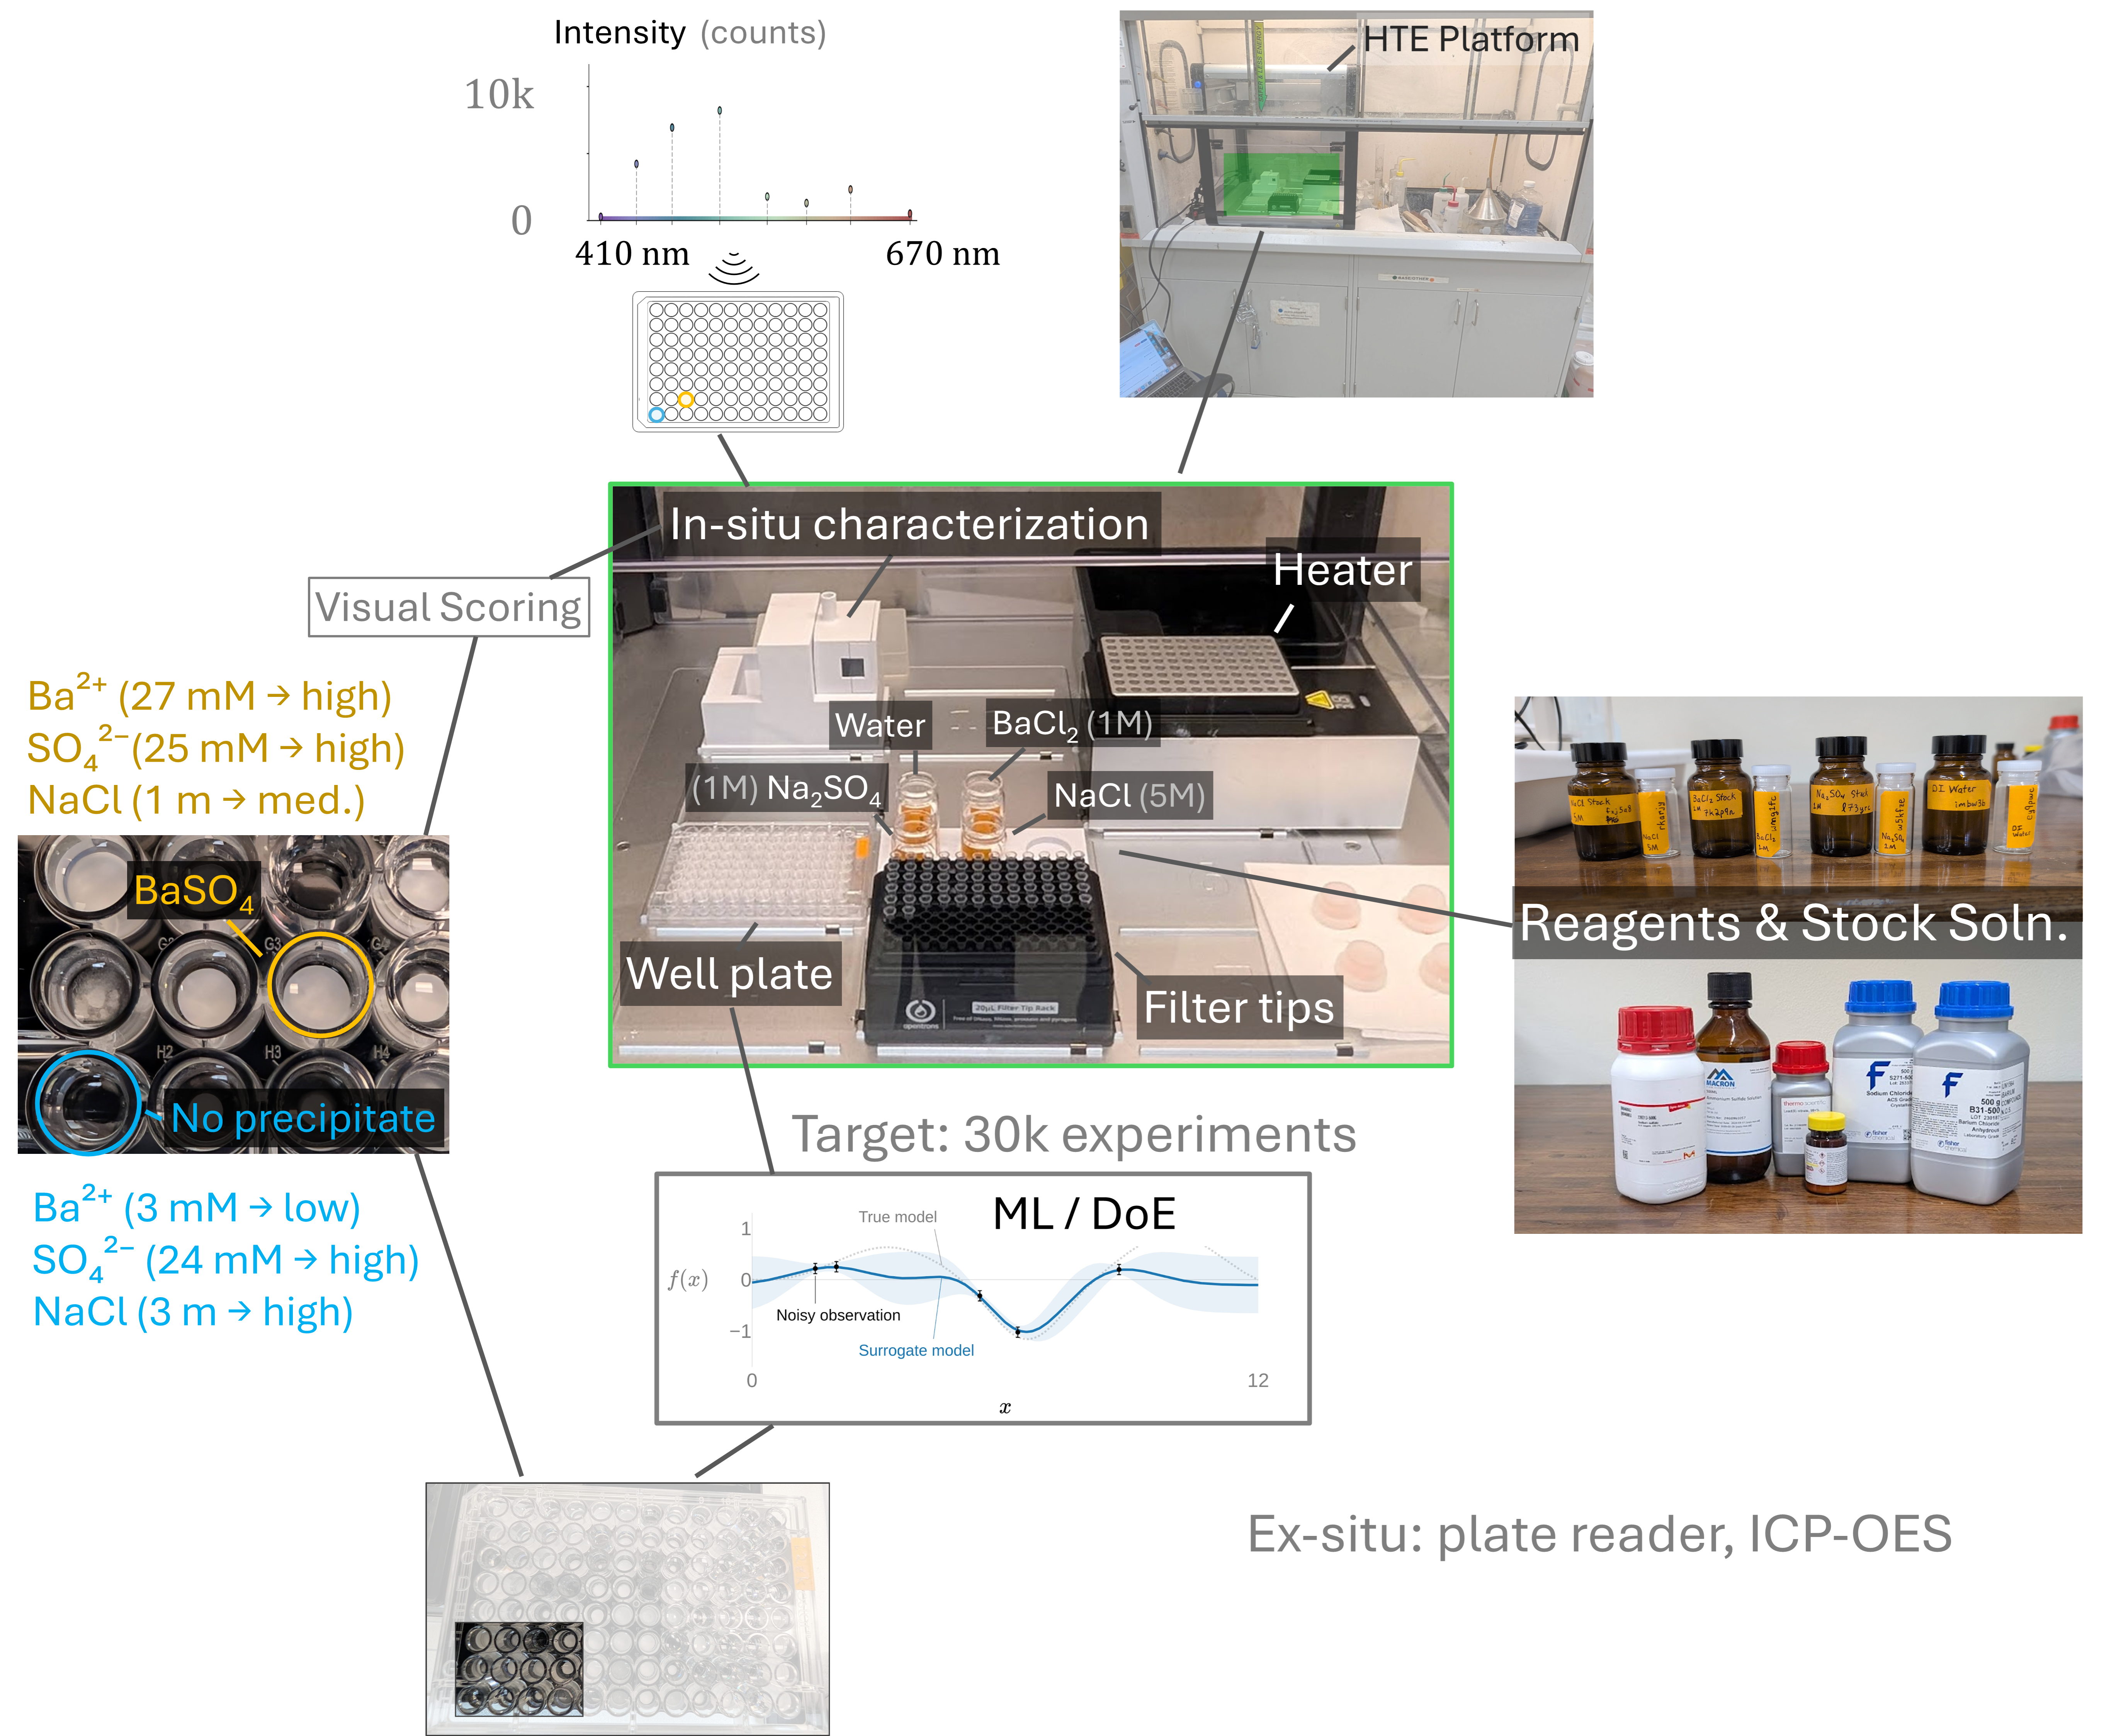
\includegraphics[width=0.55\textwidth]{./hte-platform.png}
\caption{Aim~1 high-throughput platform. Stock solutions are dispensed into 96-well plates, adaptively sampled across the 19-dimensional input space, and analyzed via in-situ spectrophotometry, in-situ overhead camera imaging, and ex-situ microplate-reader absorbance with 5\% characterized by ICP-OES. Data above were collected for BaSO$_4$ as a proof-of-concept.}
\label{fig:aim1}
\vspace{-1em}
\end{wrapfigure}

\textbf{Stock solution preparation.} Concentrated stock solutions of FeSO$_4$ (or FeCl$_2$), PbCl$_2$, NaHS, NaCl, CaCl$_2$, sodium acetate, sodium propionate, and pH buffer components (MES, HEPES, and bicarbonate) will be prepared gravimetrically in deoxygenated ultrapure water. Organic acids are introduced as their sodium salts to decouple organic acid concentration from pH. For iron(II) experiments, all Fe$^{2+}$-containing solutions will be prepared and dispensed inside a standard N$_2$ glovebox to prevent oxidation to Fe(III); critically, the OT-2 will be placed \textit{inside} the glovebox for Fe$^{2+}$ campaigns, because standard 96-well plates are not gas-tight and even trace O$_2$ can produce confounding iron oxyhydroxide precipitates within hours \cite{wang2024}. A general-purpose inert-atmosphere glovebox (being procured from PI startup funds) is sufficient; the ultradry ($<$1~ppm H$_2$O) conditions required for battery or air-sensitive organometallic work are \textit{not} needed, since all solutions are aqueous. The glovebox atmosphere will be maintained at O$_2$ $<$ 5~ppm with continuous electrochemical monitoring. Fe$^{2+}$ stocks will be prepared fresh daily from solid salts in water deoxygenated by N$_2$ sparging ($>$30~minutes) and stored sealed inside the glovebox; $\sim$10\% of preparations will be checked by 1,10-phenanthroline assay (510~nm), and batches with $>$2\% Fe$^{3+}$ will be discarded and remade. The glovebox will therefore not be compromised for more moisture-sensitive projects. Pb$^{2+}$ experiments do not require inert atmosphere and will be conducted in the fume hood.

\textbf{Experimental design.} Rather than a conventional full factorial grid, we will employ a Latin hypercube sampling (LHS) design \cite{mckay1979} to efficiently fill the 19-dimensional input space (18 independent stock-solution compositions plus temperature) with near-uniform coverage while requiring fewer total experiments than a full factorial. LHS ensures that projections onto each individual variable axis are evenly sampled, which is critical for subsequent regression of Pitzer parameters that may depend differently on each variable. For each metal system (Fe$^{2+}$, Pb$^{2+}$), we will generate approximately 2,500 unique LHS conditions spanning: metal-ion concentration (0.01--100~mM, log-spaced), sulfide concentration (0.01--50~mM, log-spaced), organic acid concentration (0--5{,}000~mg/L sodium acetate or sodium propionate), ionic strength (0.5--5~molal NaCl $\pm$ 0.5~molal CaCl$_2$), pH (4--9), and temperature (25, 60, 90~$^\circ$C). Each 96-well plate will contain a unique set of LHS-sampled conditions plus matrix-matched blanks and BaSO$_4$ positive controls. Three replicate plates will be prepared for each batch of conditions to enable statistical uncertainty quantification, yielding approximately 7,500 initial measurements per metal system ($\sim$15,000 total across both systems). An additional $\sim$15,000 measurements will be generated via adaptive follow-up (see below), bringing the grand total to approximately 30,000 experiments. All experimental metadata---timestamps, ambient temperature, humidity, solution ages, and OT-2 protocol version---will be recorded in a structured database to support reproducibility and future reanalysis.

\textbf{Adaptive follow-up via active learning.} After the initial LHS campaign, adaptive sampling will concentrate measurements near precipitation boundaries where parameter sensitivity is highest. The 19-dimensional input space (18 stock-solution compositions plus temperature) motivates a staged approach: the first $\sim$300 adaptive conditions use fully Bayesian surrogate models with sparse axis-aligned subspace priors \cite{baird2022,eriksson2021}; standard BO with scalable Gaussian process surrogates then guides selection through $\sim$1{,}000 total adaptive points; remaining experiments revert to space-filling LHS for uniform coverage. Quasi-random (Sobol) sampling will augment any stage where experimental noise impedes surrogate models. This fully Bayesian$\to$standard BO$\to$LHS strategy balances statistical efficiency with computational tractability.

\textbf{High-throughput sample preparation.} An Opentrons OT-2 robot equipped with single-channel and 8-channel pipettes (GEN2, 20--300~$\mu$L) and a heater-shaker module (25--90~$^\circ$C) will dispense stock solutions into 96-well plates, mix via orbital shaking, and incubate at target temperatures. The robot's Python API enables scripted, reproducible protocols with full logging of volumes, well positions, and timestamps.

\textbf{Detection.} A dedicated microplate reader (procured from PI startup funds) will measure absorbance at 600~nm, providing quantitative, time-resolved turbidity data. Measurements at 1, 5, 15, 60, and 240~minutes post-mixing distinguish rapid thermodynamic precipitation from slow kinetic nucleation. Visual scoring of each well as precipitate/no-precipitate serves as independent backup; both FeS (black) and PbS (black/brown) are readily visible against clear backgrounds.

\textbf{Feasibility validation (BaSO$_4$).} Feasibility has been established by proof-of-concept BaSO$_4$ experiments on one 96-well plate containing 80 Latin hypercube-sampled conditions varying Ba$^{2+}$, SO$_4^{2-}$, and NaCl. Representative plate images (e.g., wells G1, H1, F3, G3) show the expected qualitative progression from clear/faint turbidity to strongest precipitation at higher ion product. These controls validate the Aim~1 plate workflow.

\textbf{Controls and quality assurance.} Each plate includes matrix-matched blanks and BaSO$_4$ positive controls to validate detection at each ionic strength. Adhesive plate seals minimize H$_2$S off-gassing and evaporation. Disposable filter-tipped pipette tips prevent cross-contamination. A subset of the $\sim$300 ICP-OES samples (Aim~2) will include boundary conditions repeated at larger scale (5~mL vials) for validation.

\subsection{Aim 2: Pitzer-Model Comparison and Parameter Regression}

\begin{wrapfigure}{r}{0.28\textwidth}
\centering
\vspace{-1.5em}
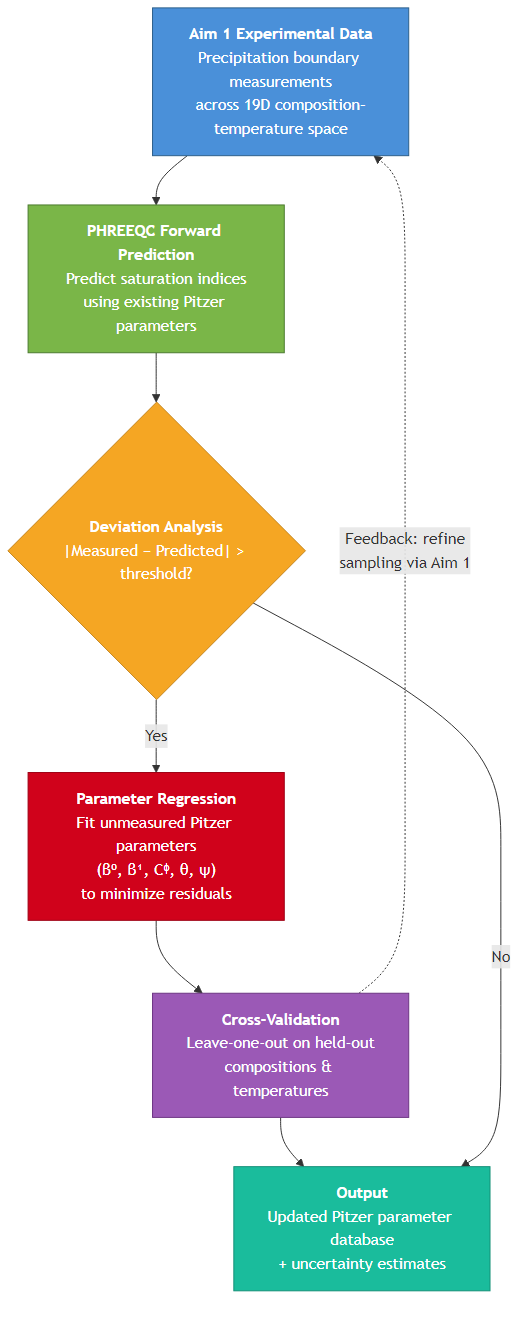
\includegraphics[width=0.26\textwidth]{aim2_pipeline.png}
\caption{Aim~2 pipeline. Experimental boundaries are compared to PHREEQC Pitzer predictions; where deviations exceed $\pm$0.2~SI, new parameters are regressed and validated.}
\label{fig:aim2}
\vspace{-1em}
\end{wrapfigure}

\textbf{Thermodynamic modeling.} For each experimental condition, we will calculate the saturation index (SI~$= \log(Q/K_{\text{sp}})$) using PHREEQC with the Pitzer database (pitzer.dat) and, where available, supplementary interaction parameters from the recent literature \cite{kan2019,wang2020,felmy2000}. The speciation calculation will explicitly account for metal--chloride complexation (e.g., FeCl$^+$, PbCl$^+$, PbCl$_2^0$, PbCl$_3^-$), metal--sulfide complexation (e.g., FeHS$^+$, FeS$^0_{\text{aq}}$), sulfide protonation equilibria (H$_2$S/HS$^-$/S$^{2-}$), and ion-pair formation---ensuring that missing Pitzer parameters are not artificially compensated by neglecting speciation \cite{felmy2000}. Wang (2024) demonstrated that fitting Pitzer coefficients for Fe--HS, Fe--Cl, and Fe--SO$_4$ pairs simultaneously---including the FeS$^0_{\text{aq}}$ stability constant---yields a mean SI error of $\pm$0.015 across 154 data points spanning 0--5~mol/kg ionic strength and 23--125~$^\circ$C \cite{wang2024}; we will adopt Wang's Fe$^{2+}$--HS$^-$ binary parameters as initial values and benchmark the Fe system against this framework and PHREEQC's \texttt{pitzer.dat}. For Fe$^{2+}$--Cl$^-$ interactions and for the Pb system more broadly, we will additionally compare to Bozau's gebo database \cite{bozau2013}, noting that Fe$^{2+}$--HS$^-$ binary Pitzer parameters are not documented in gebo and are therefore a primary target of regression in this work.

Of the $\sim$48 total parameters, 6 have prior estimates (3 Fe$^{2+}$--HS$^-$ binary from Wang 2024 \cite{wang2024} and 3 Pb$^{2+}$--Cl$^-$ temperature-dependent from Woosley \& Millero 2013 \cite{woosley2013}); the remaining $\sim$42 have no prior estimates. The 34 inorganic parameters include: Fe$^{2+}$--HS$^-$ and Pb$^{2+}$--HS$^-$ binary and mixing terms, neutral-species parameters for FeS$^0_{\text{aq}}$ and PbS$^0_{\text{aq}}$, Pb$^{2+}$--SO$_4^{2-}$ and PbCl$_2^0$ terms, and metal--hydroxide corrections \cite{felmy2000,kan2019,mgaidi1991}. The $\sim$14 organic acid--metal parameters comprise binary terms ($\beta^{(0)}$, $\beta^{(1)}$, $C^\phi$) for Fe$^{2+}$-- and Pb$^{2+}$--acetate and --propionate (12 total) plus sulfide--carboxylate mixing terms ($\sim$2). Organic-organic mixing parameters (e.g., $\theta$(OAc$^-$--Prop$^-$)) are excluded because organic acid concentrations in produced waters are 2--4 orders of magnitude below the dominant inorganic anions (Cl$^-$, SO$_4^{2-}$), making their mutual interaction contributions negligible compared to the metal--organic cross terms \cite{pitzer1974}.

\textbf{Sensitivity analysis and parameter prioritization.} To assess parameter identifiability, we computed analytical derivatives of the Pitzer equations---the same functional forms implemented in PHREEQC---yielding $\partial\mathrm{SI}/\partial p_j$ across six condition classes (FeS and PbS at low, medium, and high ionic strength; Figure~\ref{fig:param_sens}). This approach parallels perturbed-parameter PHREEQC simulations using analytical derivatives \cite{pitzer1973}. All 48 parameters are identifiable ($|\partial\mathrm{SI}/\partial p| > 0.05$), with a hierarchical structure: binary terms ($\beta^{(0)}$, $\beta^{(1)}$, $C^\phi$) dominate direct ion interactions, mixing terms ($\theta$, $\psi$) gain influence with ionic strength, and neutral-species terms ($\lambda$, $\zeta$) matter when neutral complexes are favored. This sensitivity structure validates the proposed phased fitting strategy and guides adaptive follow-up sampling.

\begin{figure}[!htb]
\centering
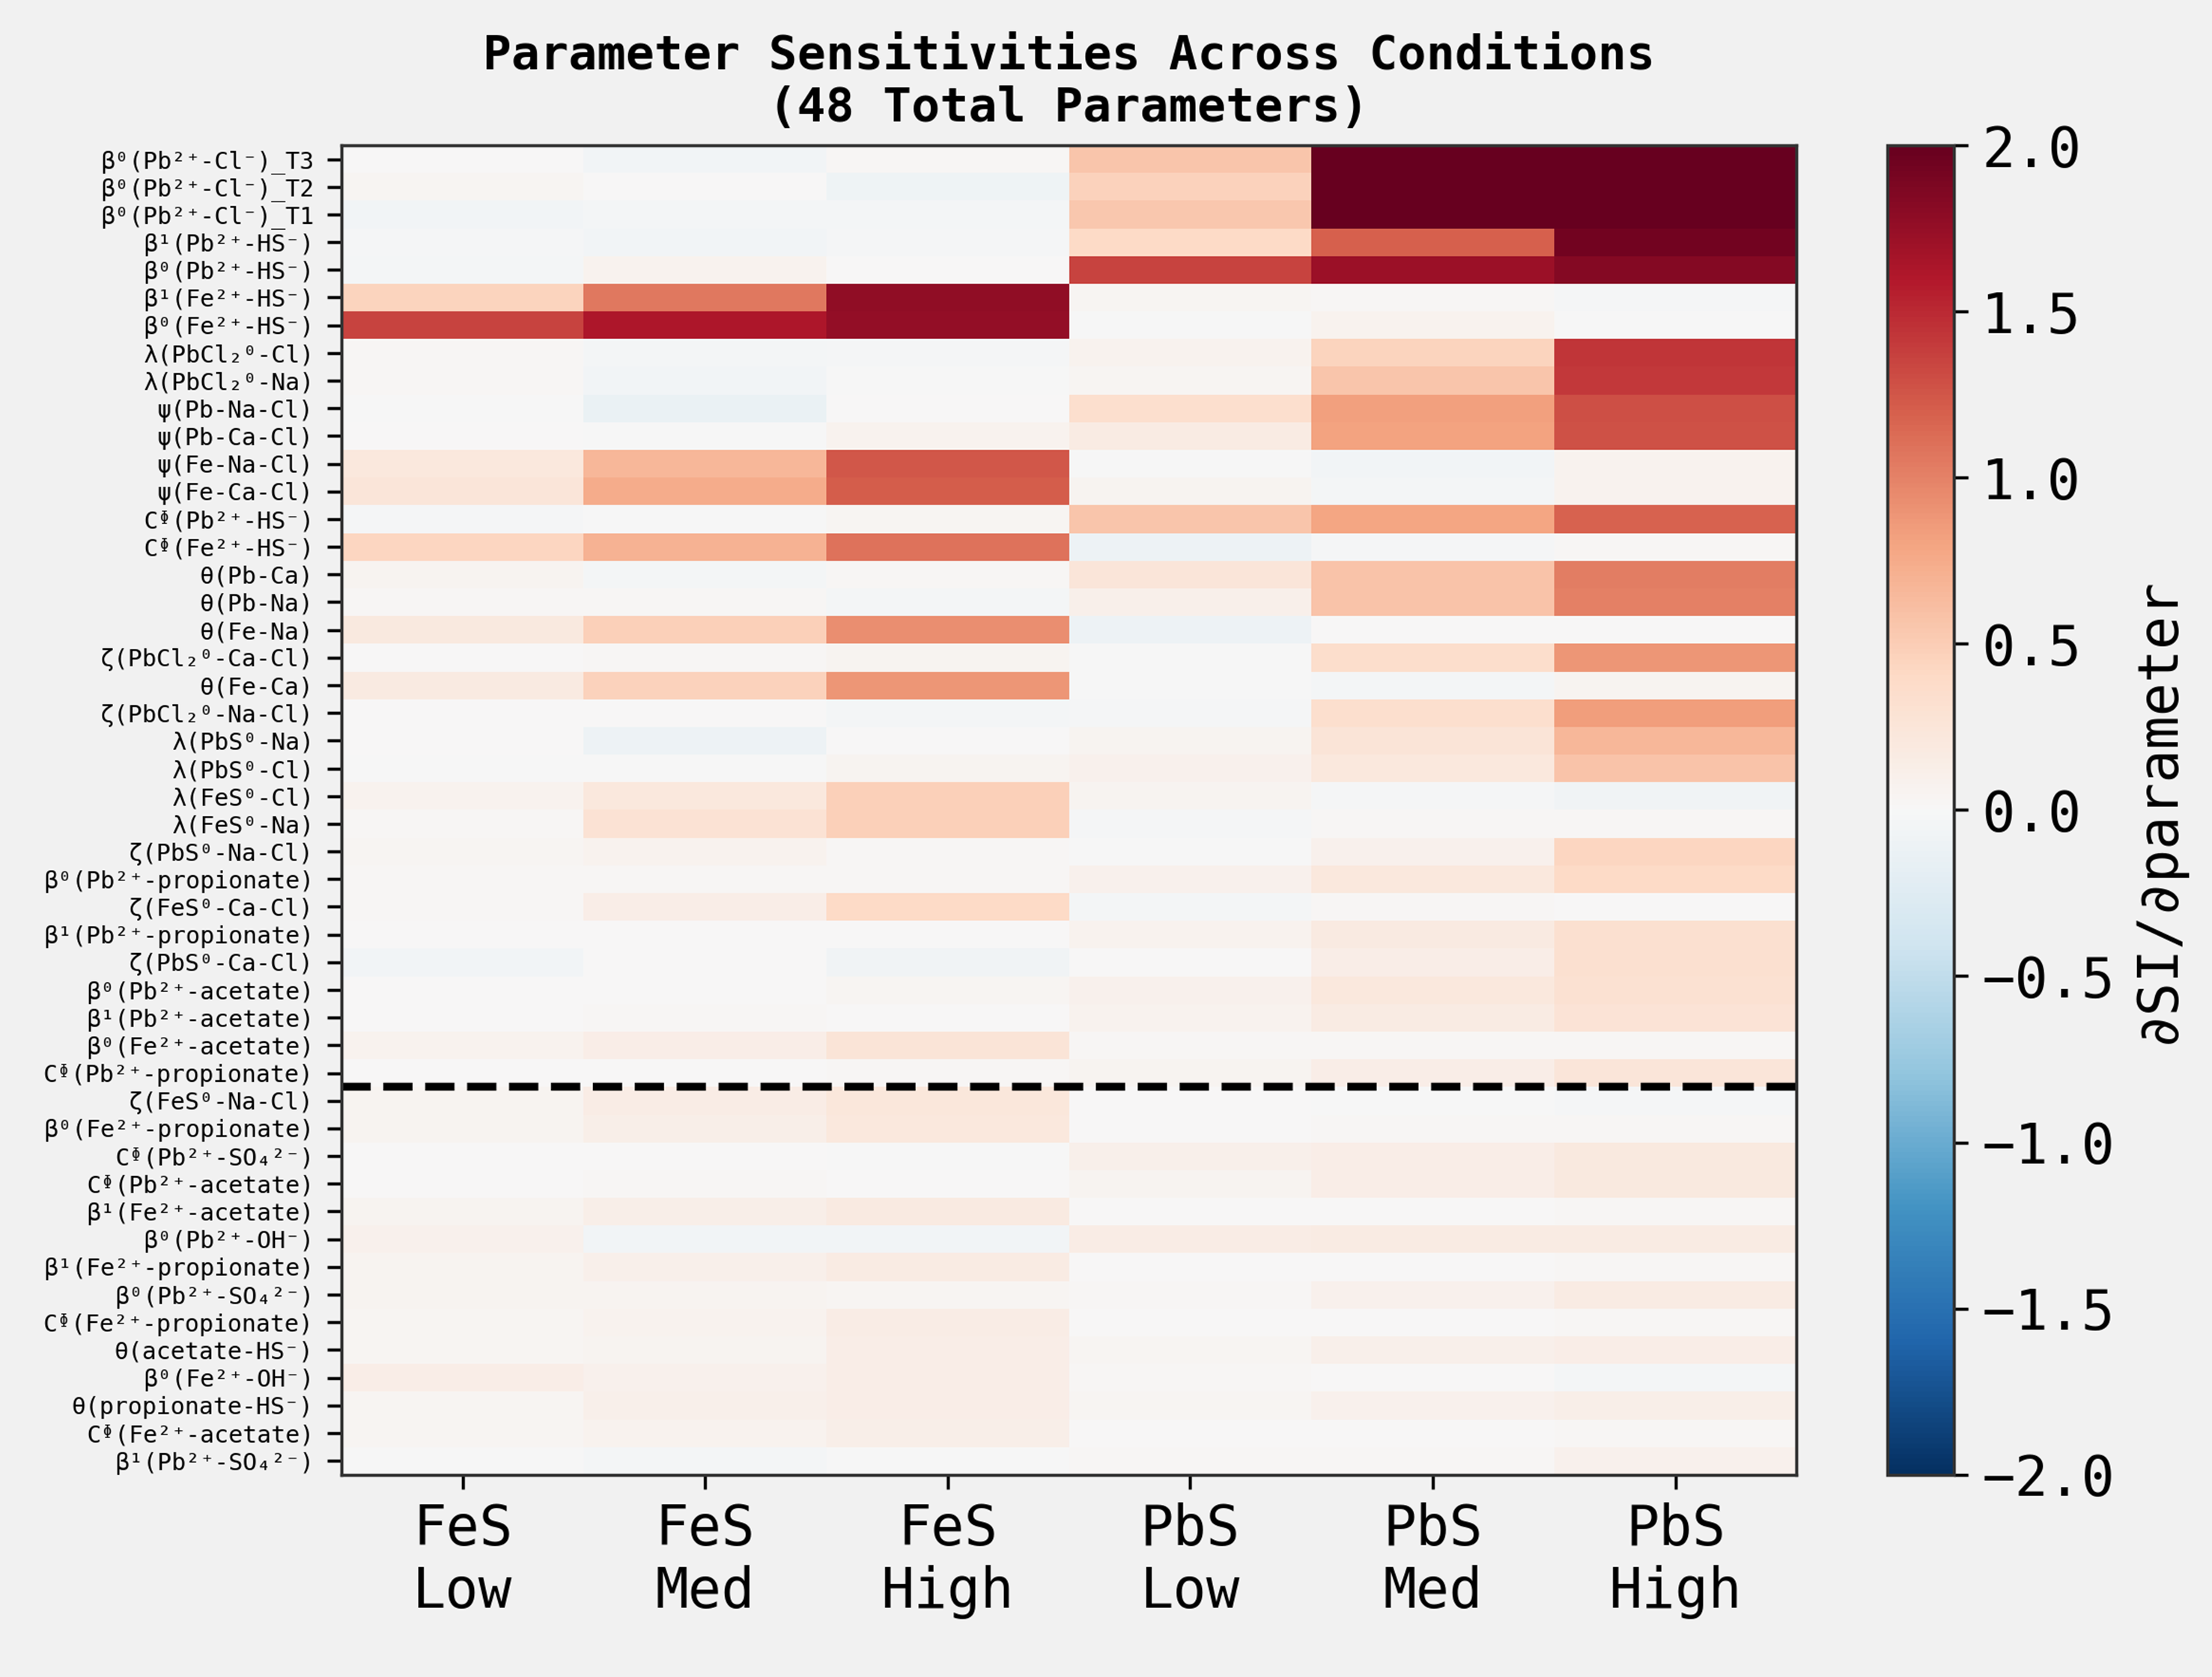
\includegraphics[width=0.65\textwidth]{parameter-sensitivities-48.png}
\caption{Parameter-sensitivity heatmap ($\partial\mathrm{SI}/\partial p_j$) computed from analytical derivatives of Pitzer equations \cite{pitzer1973}. Rows: 48 target parameters; columns: six condition classes (FeS/PbS at low, medium, high ionic strength). All parameters show $|\partial\mathrm{SI}/\partial p| > 0.05$, confirming identifiability.}
\label{fig:param_sens}
\end{figure}

Preliminary PHREEQC calculations confirm this gap (Figure~\ref{fig:phreeqc_si}). Saturation indices computed across 0.1--5.0~molal NaCl at 25~$^\circ$C show a 1.3~SI-unit response for BaSO$_4$ (well-parameterized Pitzer model), but only 0.1 and 0.8~SI for FeS and PbS (Davies equation only). Galena is not defined in standard PHREEQC databases. These flat Davies curves are unreliable above $I \approx 0.5$~molal.

\begin{figure}[!htb]
\centering
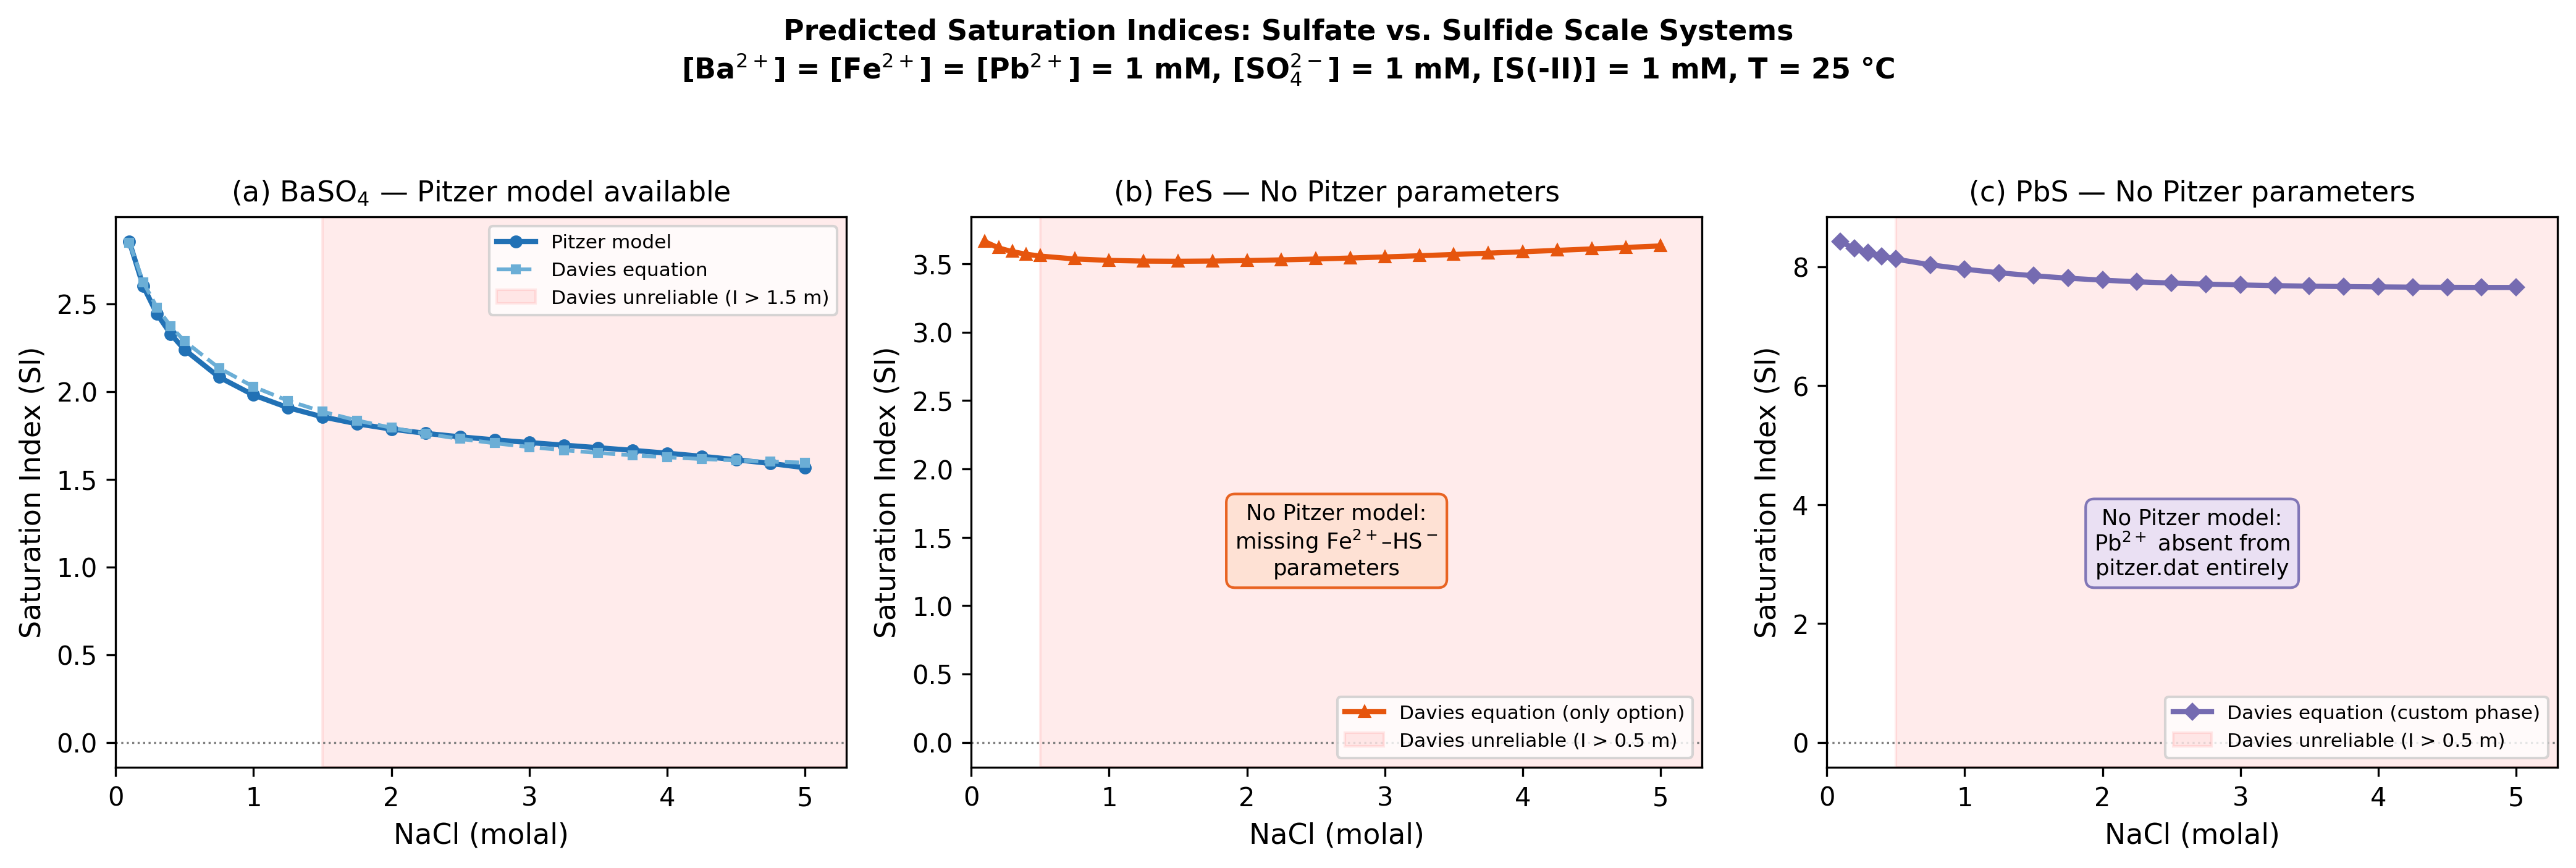
\includegraphics[width=0.85\textwidth]{../preliminary_results/phreeqc_si_comparison.png}
\caption{Predicted saturation indices vs.\ NaCl concentration (0.1--5.0~molal) at 25~$^\circ$C for (a)~BaSO$_4$ (Pitzer model), (b)~FeS (Davies equation only), and (c)~PbS (Davies equation; Pb$^{2+}$ absent from \texttt{pitzer.dat}). Flat sulfide curves above $I \approx 0.5$~molal reflect the Davies limitation. \textbf{This gap is the target of the proposed research.}}
\label{fig:phreeqc_si}
\end{figure}

\FloatBarrier

% add reference to next figure, describing and incorporating it into the narrative

Figure \ref{fig:si-response} quantifies this contrast: the well-parameterized BaSO$_4$ system shows 1.3~SI units variation versus only 0.1 (FeS) and 0.8 (PbS) for the Davies-equation sulfide systems.

\begin{wrapfigure}{r}{0.5\textwidth}
\centering
\vspace{-1.5em}
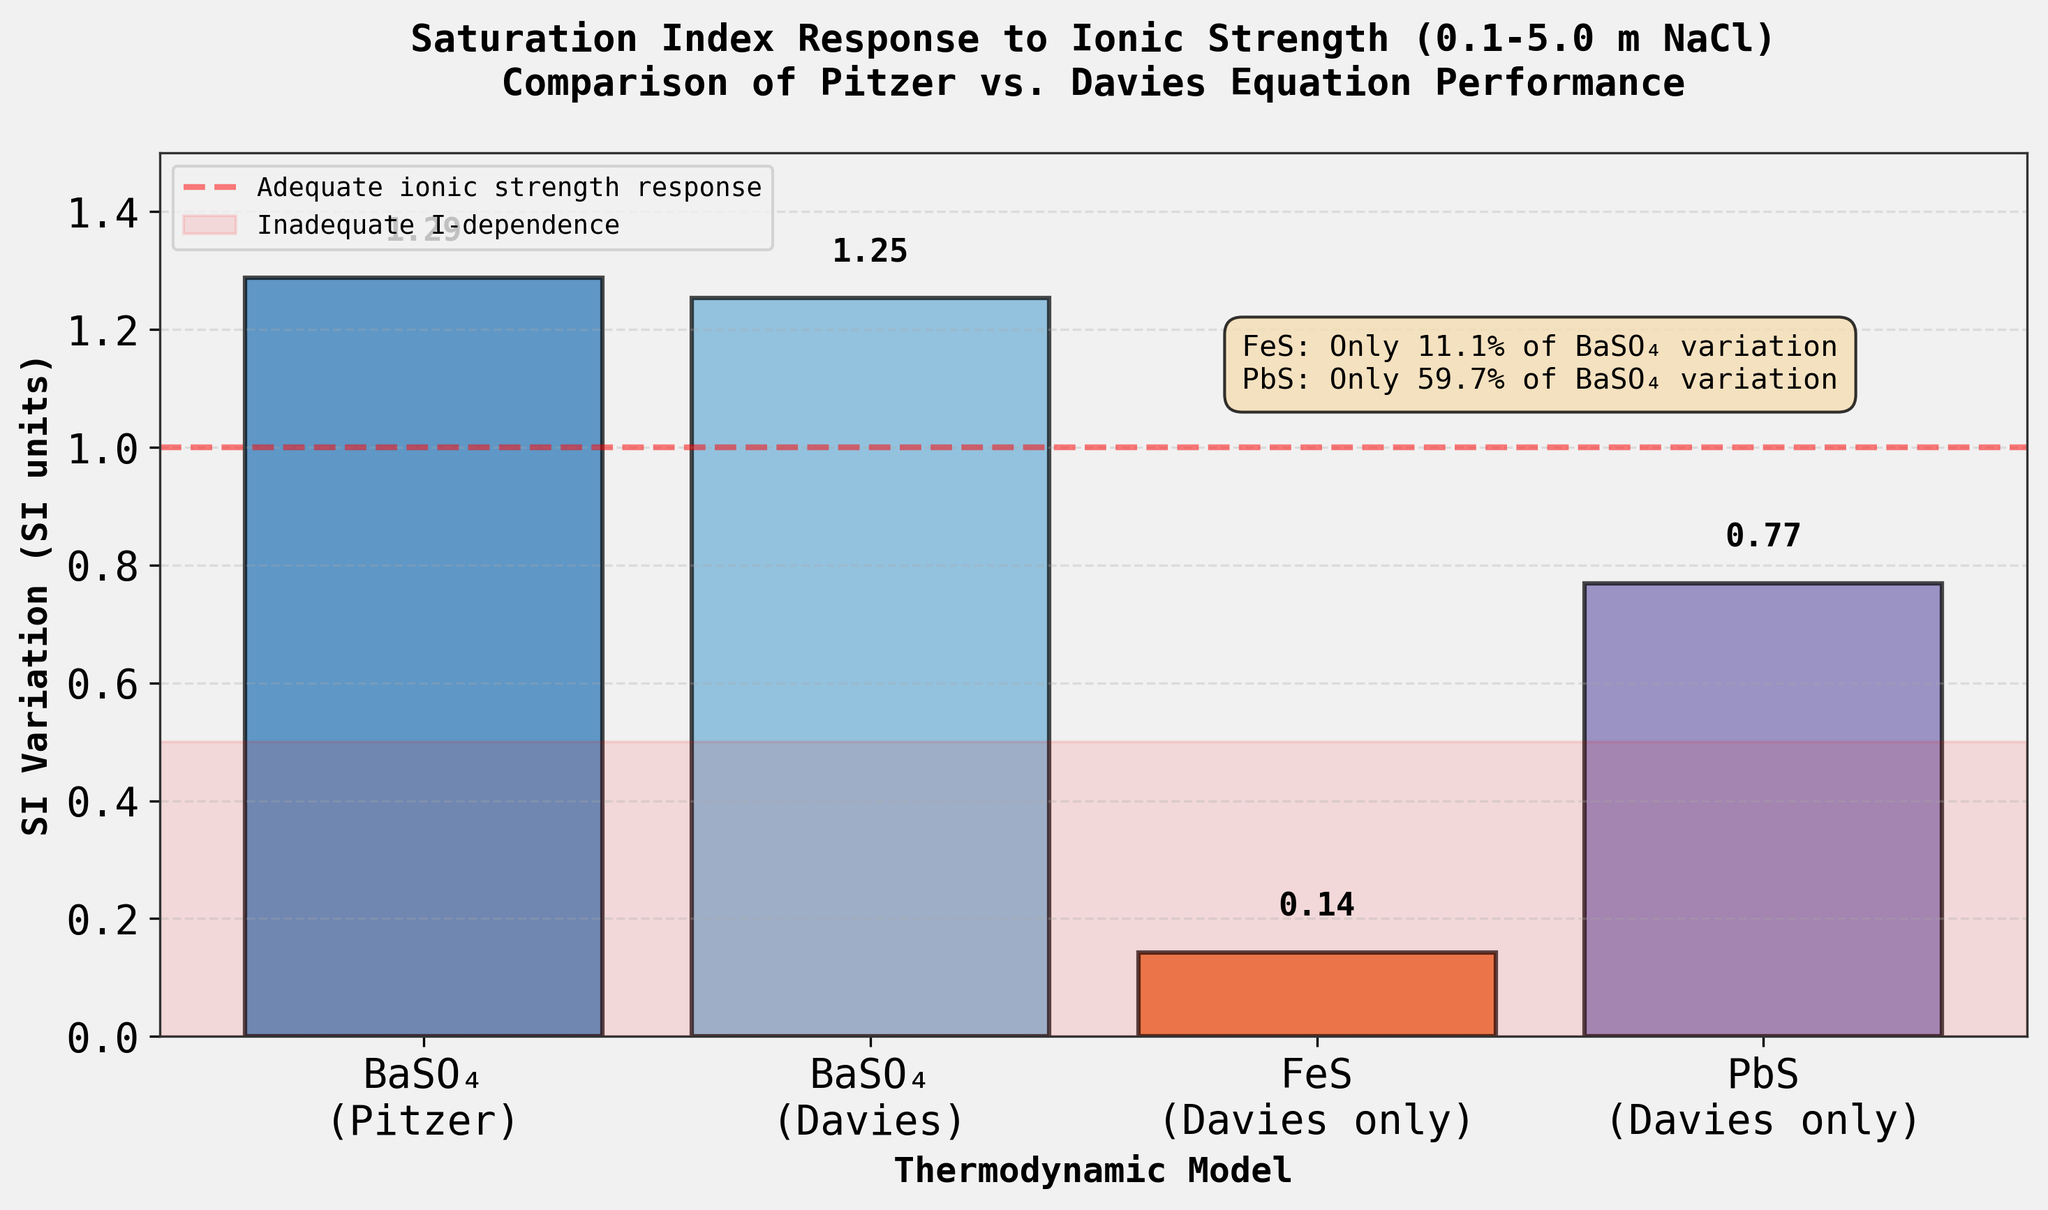
\includegraphics[width=0.45\textwidth]{../preliminary_results/saturation-index-response.png}
\caption{The Davies activity model inadequately captures the ionic strength dependence of sulfide mineral saturation. The bar chart shows the total variation in the saturation index (SI) from PHREEQC simulations over an ionic strength range of 0.1-5.0 m NaCl, comparing BaSO$_4$ (Pitzer and Davies models) with FeS and PbS (Davies model only). The substantially smaller SI variation for FeS and PbS relative to the parameterized BaSO$_4$-Pitzer system highlights the failure of the standard Davies model to predict mineral behavior in high-salinity sulfide systems.}
\label{fig:si-response}
\vspace{-1em}
\end{wrapfigure}

\textbf{Comparison framework.} The binary outcome (precipitation observed vs.\ not) at each condition defines an empirical boundary, compared to the model-predicted SI~$= 0$ contour. Systematic offsets---e.g., the model predicting supersaturation where no precipitate is observed---implicate missing or inaccurate interaction parameters.

\textbf{Image analysis.} All plate images will be archived with associated metadata. Manual annotation of precipitate/no-precipitate provides a ground-truth dataset; in parallel with the manual annotation, an OpenCV classifier \cite{bradski2000} will be developed and trained on manual annotations (e.g., $>$2,000 wells).

\textbf{Parameter regression.} Guided by the sensitivity structure in Figure~\ref{fig:param_sens}, where the average deviation between predicted and observed boundaries exceeds $\pm$0.2~SI, we will regress the full set of $\sim$48 parameters using weighted nonlinear least-squares optimization with ridge regularization to mitigate parameter correlations; model complexity will be assessed via the Bayesian Information Criterion (BIC). Initial values will be drawn from Pitzer's combining rules where available. As a core component of the parameter regression, $\sim$300 conditions ($\sim$5\% of unique compositions) spanning the ionic-strength range will be selected for quantitative dissolved-metal analysis via ICP-OES (\$24/sample, funded from PI startup), providing continuous concentration data essential for constraining individual Pitzer parameters that are correlated along the saturation-index surface. Binary precipitation data alone constrain only the SI~$= 0$ contour; continuous dissolved-metal concentrations provide information about the magnitude of supersaturation and are therefore critical for resolving parameter correlations.

\textbf{Validation.} The regressed parameters will be validated using held-out data (20\% of the dataset) and literature data where available. We will employ 5-fold cross-validation \cite{arlot2010} and extrapolatory ``challenge'' splits (e.g., withholding all data above $I > 3$~molal) to assess whether regressed parameters generalize beyond the training domain, with challenge regimes selected to stress the highest-sensitivity condition blocks in Figure~\ref{fig:param_sens}. A successful outcome is defined as reducing SI deviation to $< \pm$0.1~SI across the full parameter space.

\subsection{Timeline}

\textbf{Year~1} (Months 1--12): Stock solution preparation and protocol validation (Months 1--3); FeS precipitation boundary mapping at 25~$^\circ$C across ionic strength and pH (Months 3--10); begin PHREEQC modeling and active-learning-guided follow-up experiments (Months 8--12). \textbf{Year~2} (Months 13--24): Pb$^{2+}$ precipitation mapping at 25--90~$^\circ$C (Months 13--18); temperature-dependent FeS measurements and adaptive sampling near identified precipitation boundaries (Months 13--18); complete Pitzer-model comparisons and parameter regression (Months 15--21); manuscript preparation and submission (Months 18--24).

\textbf{Fitting strategy.} We will adopt a hierarchical fitting approach as the primary regression strategy: first fix Pb$^{2+}$--Cl$^-$ and Pb$^{2+}$--SO$_4^{2-}$ parameters at published values \cite{felmy2000,woosley2013,mgaidi1991} and adopt Wang's (2024) Fe$^{2+}$--HS$^-$ binary coefficients as initial values \cite{wang2024}, reducing the initial free parameter count to $\sim$36; sulfide-specific and organic acid--metal terms will be regressed hierarchically, with additional parameters released sequentially as the dataset grows and parameter identifiability improves. If Fe$^{2+}$ oxidation proves difficult to control despite glovebox preparation, we will prioritize the PbS system (which requires no inert atmosphere) and treat FeS as a secondary campaign once the oxidation-control protocol is validated, reducing the active parameter set to $\sim$24. A dedicated microplate reader will be procured from PI startup funds for quantitative absorbance measurements.

\section{Expected Results and Impact}

Existing Pitzer models should predict FeS and PbS precipitation accurately at $I < 1$~molal but deviate above $\sim$2~molal due to missing mixing terms ($\theta_{ij}$, $\psi_{ijk}$) \cite{kan2019}. The Pb$^{2+}$ system represents the most severe gap \cite{felmy2000}. We anticipate models will overpredict supersaturation because unmeasured repulsive interactions between scale-forming and matrix cations effectively increase sulfide-mineral solubility. The framework will also reveal how petroleum-derived organic acids shift sulfide precipitation boundaries---critical for produced waters where organic acid concentrations vary by two orders of magnitude. The validated parameters will be formatted for direct import into PHREEQC \texttt{pitzer.dat}, ScaleSoftPitzer, and OLI databases, extending Pitzer theory to sulfide systems for the first time and enabling downstream applications in sour (H$_2$S-bearing) reservoir geochemistry \cite{kan2019}. The methodology transfers to other petroleum-relevant scale systems (CaCO$_3$, SrSO$_4$), and preliminary data will support larger proposals (NSF CAREER).

\section{Student Training Plan}

This project will support one master's-level graduate student and two part-time undergraduate researchers over the two-year grant period. BYU's Department of Mechanical Engineering enrolls a large M.S.\ cohort, and master's students regularly complete thesis-based research within 2~years---well-matched to the ACS PRF timeline. The M.S.\ student will begin in Year~1 and will conduct FeS and PbS precipitation experiments, PHREEQC thermodynamic modeling, and Pitzer parameter regression. The student will receive training in four key areas: (1)~\textit{inorganic aqueous chemistry}, including solution thermodynamics, activity-coefficient models, and metal-ion speciation; (2)~\textit{automated experimentation}, including robotic sample preparation (Python/Opentrons API), experimental design, and high-throughput data collection; (3)~\textit{computational modeling}, including PHREEQC thermodynamic calculations, nonlinear parameter regression, and data visualization; and (4)~\textit{scientific communication}, including thesis writing, conference presentations, and data management. Students will take elective courses in chemical thermodynamics, instrumental analysis, optimization, and statistical learning across BYU departments.

Undergraduate researchers will contribute to stock solution preparation, data collection, and image analysis during the academic year and summer. BYU has a strong culture of undergraduate research participation, and these positions will provide hands-on experience with quantitative inorganic chemistry techniques and exposure to modern research methods including robotic laboratory automation and computational thermodynamics---competencies increasingly valued in industrial and academic careers. All students will present their work at ACS national or regional meetings and will be co-authors on resulting publications.

Given the PI's newness to aqueous geochemistry and sulfide chemistry, this project will use targeted consultations. \textbf{Prof. Milad Abolhasani} (North Carolina State University Chemical and Biomolecular Engineering) has agreed to bi-annual meetings focused on high-throughput experimental design and robotic workflows for chemistry applications. \textbf{Prof. Barry Bickmore} (BYU Geology) can advise on mineral--water geochemistry and Pitzer-database workflows. \textbf{Prof. Dean Wheeler} (BYU Chemical Engineering) is an additional planned consultant for broader thermodynamics and experimental strategy. This mentorship structure aligns with planned submission to ACS PRF Panel 2 (Geochemistry and Biogeochemical Cycling). The PI will present initial findings at a forum such as the Goldschmidt Conference.

%TC:ignore
\vspace{1em}
\noindent\textit{Word count (body text, excluding abstract, captions, and references): \wordcount{} / 4{,}000}
%TC:endignore

% \section{References}

\begin{singlespace}
\bibliographystyle{unsrtnat}
\bibliography{references_final}
\end{singlespace}

\end{document}
